\begin{appendices}

\newpage
\section{Diagram sieciowy architektury}
\label{app:network_diagram_app}
\begin{figure}[H]
\begin{center}
    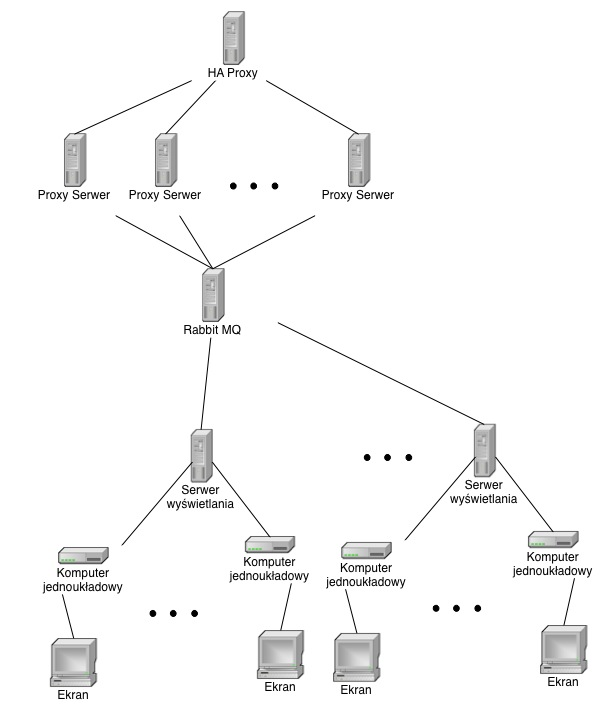
\includegraphics[width=\linewidth]{network_diagram}
\end{center}
\caption{Diagram sieciowy.}
\label{fig:network_diagram1}
\end{figure}



\newpage
\section{Diagram komponentów gry PONG}
\label{app:netwo}
\begin{figure}[H]
\begin{center}
    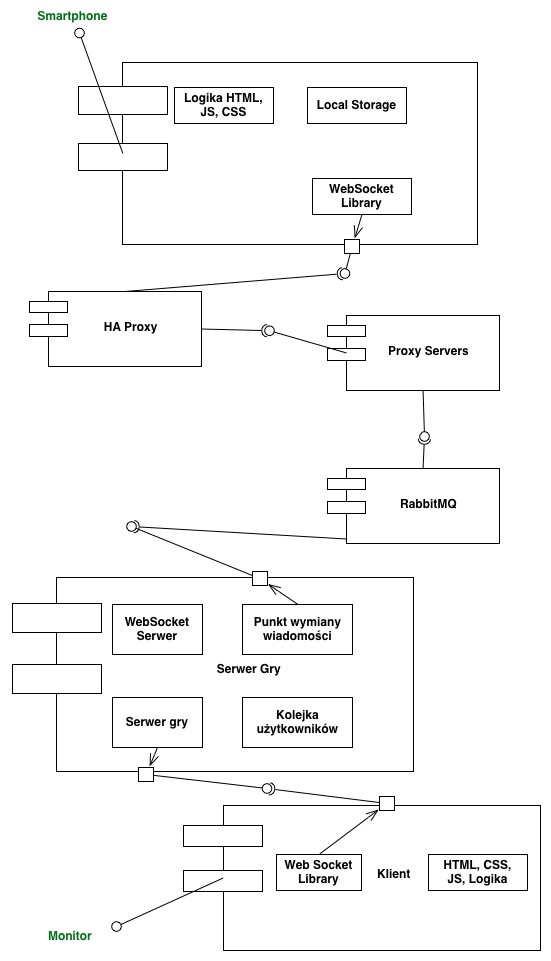
\includegraphics[scale=0.5]{pong_components_diagram}
\end{center}
\caption{Diagram komponentów w grze PONG}
\label{fig:network_diagram}
\end{figure}



\newpage
\section{Diagram komponentów sterowania ekranem}
\label{app:netwo}
\begin{figure}[H]
\begin{center}
    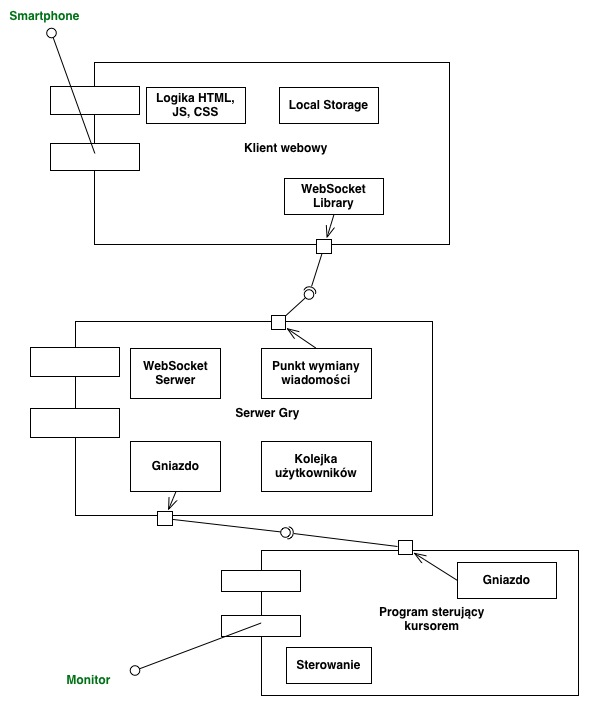
\includegraphics[width=\linewidth]{control_components_diagram}
\end{center}
\caption{Diagram komponentów do sterowania zdalnym ekranem}
\label{fig:network_diagram}
\end{figure}




\newpage
\section{Program serwera w kliencie}
\label{app:server_c}
\lstinputlisting[language=c]{assets/src/server.c}
Powyższy fragment otwiera gniazdo na porcie 8081 i czeka na połączenie z serwera gry. Po pomyślnym połączeniu ze zdalnym hostem wykonywana jest instrukcja \lstinline|pipe|. Jest to jeden z mechanizmów komunikacji międzyprocesowej umożliwiający wymianę danych pomiędzy procesami. Funkcja jako argument dwuelementową tablicę liczb całkowitych, po pomyślnym wykonaniu polecenia tablica będzie zawierała dwa nowe deskryptory pliku. Pierwszy element tablicy jest deskryptorem pliku z którego można czytać, drugi natomiast przeznaczony jest do wpisywania.
\\
Instrukcja \lstinline|fork| tworzy nowy proces, oraz kończy swoje działanie zwracając następujące wartości:
\\
\begin{itemize}
	\item PID potomka w procesie macierzystym
	\item 0 w procesie potomnym
\end{itemize}
\\
W dalszej części kodu źródłowego programu znajduje się instrukcja warunkowa oddzielająca część wykonywaną przez proces rodzica i proces dziecka. 
\\
W części wykonywanej przez proces dziecka, zamykany jest nieużywany deskryptor. Proces ten jest odpowiedzialny jest za otworzenie programu do którego będą na standardowe wejście wpisywane komunikaty dotyczące urządzeń wejścia. Instrukcja \lstinline|dup2| duplikuje deskryptor pliku. W przypadku zaprezentowanym w powyższym fragmencie pliku zamyka deskryptor pliku w potoku, \lstinline|STDIN_FILENO| staje się niejako aliasem zamkniętego deskryptora. Przez co wyjściem stworzonego potoku nie jest pierwszy element tablicy \lstinline|uinputPipe|, ale standardowe wejście. Dzięki temu dane wpisane do \lstinline|uinputPipe[1]| trafiają wprost na standardowe wejście procesu dziecka.
\\
W części rodzica, podobnie jak w procesie dziecka zamykany jest nieużywany deskryptor, oraz za pomocą instrukcji \lstinline|read| sczytywane są dane wysłane do gniazda na porcie 8081, a następnie poprzez potok przesyłane na standardowe wejście procesu dziecka.
		


\newpage
\section{X Window System}
\label{app:X Window System}
X Window graficzny system okien:
\begin{itemize}
	\item oparty o architekturę klient-serwer
	\item niezależny od systemu operacyjnego na jakim uruchomiony jest system okien
	\item oparty o prokół TCP/IP
\end{itemize}

\begin{description}
	\item[Co to jest X serwer?] \hfill \\
		X-Serwer jest to aplikacja komunikująca się z pośrednio z kartą graficzną, myszką, monitorem etc. Udostępnia okno na, którym mogą zostać wyświetleni klienci systemu okien.
	\item[Co to jest X klient?] \hfill \\
Używa okna udostępnionego przez X Serwer do wyświetlenia aplikacji. Nie komunikuje się z kartą graficzną, czy urządzeniami wejśica.

\begin{figure}[H]
\begin{center}
    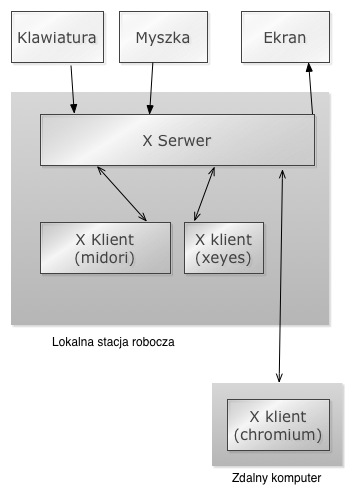
\includegraphics[scale=0.85]{x_diagram}
\end{center}
\caption{Diagram przedstawiający działanie systemu okien X.}
\label{fig:}
\end{figure}

		
\end{description}



\section{Zawartość CD}

The contents...

\end{appendices}
